\documentclass[a4paper,12pt]{scrartcl}
\usepackage{hyperref}
\usepackage{url}            % simple URL typesetting
\usepackage{booktabs}       % professional-quality tables
\usepackage{amsfonts}       % blackboard math symbols
\usepackage{amsmath}
\usepackage{nicefrac}       % compact symbols for 1/2, etc.
\usepackage{microtype}      % microtypography
\usepackage{tabto}
\usepackage{tikz}
\usepackage{graphicx}
\usepackage{longtable}
\usepackage{lmodern}
\usepackage{listings}
\usepackage[T1]{fontenc}
\usepackage[utf8]{inputenc}
\usepackage{forest}
\definecolor{folderbg}{RGB}{124,166,198}
\definecolor{folderborder}{RGB}{110,144,169}

\def\Size{4pt}
\tikzset{
  folder/.pic={
    \filldraw[draw=folderborder,top color=folderbg!50,bottom color=folderbg]
      (-1.05*\Size,0.2\Size+5pt) rectangle ++(.75*\Size,-0.2\Size-5pt);  
    \filldraw[draw=folderborder,top color=folderbg!50,bottom color=folderbg]
      (-1.15*\Size,-\Size) rectangle (1.15*\Size,\Size);
  }
}




\title{ROZPOZNAWANIE KOTKÓW OD PIESKÓW}
\author{Michał Skibiński (260352)}
\date{30.05.2022}

\begin{document}

\maketitle

\section{Wstęp}
Przedmiotem projektu jest zadanie klasyfikacji binarnej (klasyfikacji kotów oraz psów).
do rozwiązania problemu posłużyłem się \textbf{konwolucyjną siecią neuronową (CNN)}.
Ponieważ sieci neuronowe operują na macierzach, są one szczególnie wydajne przy pracy z obrazami, 
które tak naprawde są macierzami pikseli. \\
Rozwiązanie zaprojektowałem  w języku \textit{python} używając biblioteki \textit{tensorflow}.\\
Zdecydowałem się na język programowania \textit{python}, ze względu na jego prostotę, 
niezawodność oraz wielorakość bibliotek ogólno-dostępnych. \\
Bibliotekę \textit{tensorflow} wybrałem ze względu na możliwość 
wykonywania złożonych operacji na sieciach neuronowych, przy użyciu stosunkowo
niewielkiej ilości kodu. Oprócz tego biblioteka ta działa bardzo efektywnie,
 oraz została do niej napisana bogata dokumentacja.\\

\newpage{}
\section{Model}


\subsection{Przygotowanie danych}
aby przygotować dane kolejno:
\begin{enumerate}

    \item napisałem algorytm do odczytywania zdjęć z zadanego folderu i tworzeniu folderu plików z podziałem na \textbf{dane testowe i treningowe} oraz klasy, tak by strukrura wyglądała następująco: \\
    \begin{forest}
        for tree={
          font=\ttfamily,
          grow'=0,
          child anchor=west,
          parent anchor=south,
          anchor=west,
          calign=first,
          inner xsep=7pt,
          edge path={
            \noexpand\path [draw, \forestoption{edge}]
            (!u.south west) +(7.5pt,0) |- (.child anchor) pic {folder} \forestoption{edge label};
          },
          before typesetting nodes={
            if n=1
              {insert before={[,phantom]}}
              {}
          },
          fit=band,
          before computing xy={l=15pt},
        }  
      [input for model
        [train
          [cats (3830 zdjęć)
          ]
          [dogs (1915 zdjęć)
          ]
        ]
        [test
            [cats (958 zdjęć)
            ]
            [dogs (479 zdjęć)
            ]
        ]
      ]
      \end{forest}\\
      ilość danych testowych ustawiłem na 20 procent.
    \item usunąłem różnicę w ilości fotografii kotów i psów (ważne aby sieć neuronowa miała tyle samo danych z każdej z klas) 
    \item dokonałem \textbf{normalizacji danych} - przeskalowałem wartości pikseli tak by pochodziły z zakresu [0,1)
    \item ustandaryzowałem dane - wszystkie zdjęcia przeskalowałem do rozmiarów [224 x 224] px.
    \item zrezygnowałem z użycia \textbf{PCA} ponieważ redukcja wymiarów wiązała się ze zbyt dużą utratą danych. 
      
  \end{enumerate}
\subsection{Budowa modelu}
w fazie budowania modelu, inspirowałem się dotychczasowymi modelami do rozwiązania problemu.
Zanim pojawił się finałowy model stworzyłem ok 10 innych modeli, każdy był usprawnieniem poprzedniego.
skupiłem się na \textbf{funkcjach aktywujących} dla poszczególnych warstw oraz liczbie ich liczbie.\\\\

włsności modelu:
\begin{itemize}
  \item wejście dla modelu: macierz o rozmiarach (224 x 224 x 3) - gdzie 3 wynika z reprezentacji pikseli poprzez RGB 
  \item liczba warstw ukrytych: 20 
  \item wyjście: wartość 0 lub 1 (0 - dla psa, 1 - dla kota) 
  \item metoda optymalizacji:  \textbf{stochastyczny spadek gradientu(SGD)} z prędkością nauki = 0.0001
  \item funkcja strat:  binarna entropia krzyżowa
  \item ilość generacji(epok):  20
  \item populacja w każdej generacji: 60
  \item \textbf{funkcja regularyzacji}: l2 (bez regularyzacji występowało \textbf{przetrenowanie modelu})
\end{itemize}  
dla podanych parametrów zbudowane zostały medele, w których kolejno użyte zostały następujące metody optymalizacji
\begin{itemize}
  \item metoda spadku gradientu - (od SGD różni się tym, że nie używa losowości.)
  \item metoda Adam - bazuje na stochastycznym spadku gradientu, ale jest oparta na adaptacyjnym szacowaniu momentów pierwszego i drugiego rzędu
  \item metoda stochastycznego spadku gradientu - (metoda, która pojawiła się w finalnym modelu)
\end{itemize}  
poza tym każdy z modelów uruchomiłem dla danych poddanych PCA oraz dla danych nie poddanych PCA.
\subsection{Przebieg treningu}

\begin{figure}[h]
  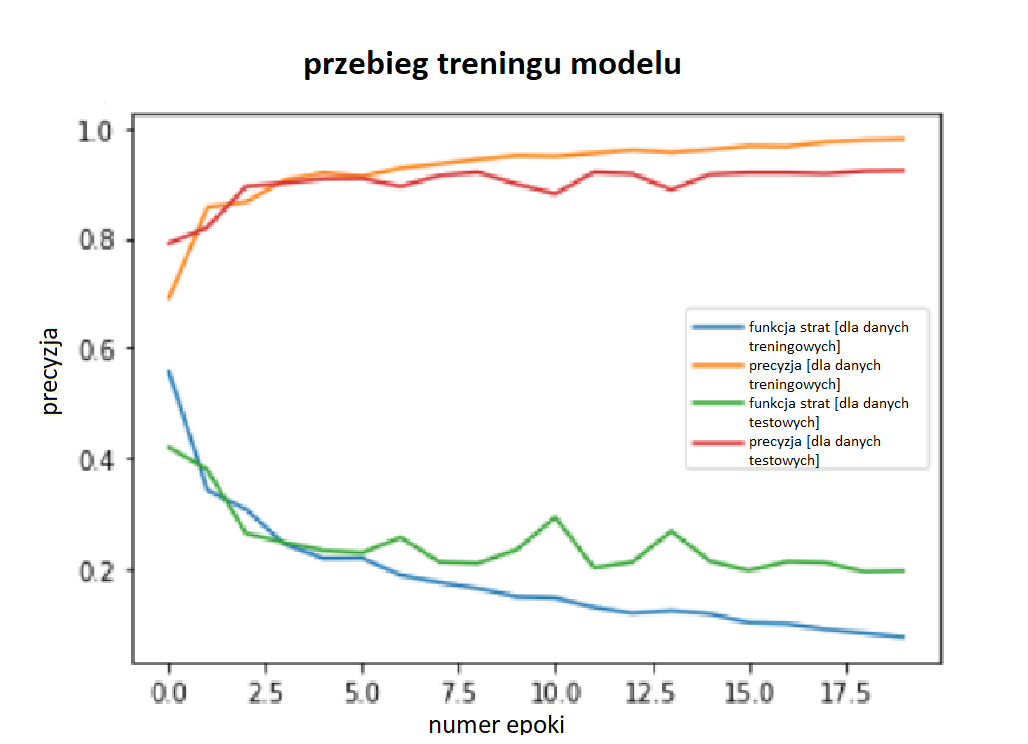
\includegraphics[width=\linewidth]{TRENINNG.png}
\end{figure}
\newpage{}
\section{Wyniki}
\subsection{Jakość modelu}
po skończonym treningu precyzja:
\begin{itemize}
\item dla danych treningowych wynosiosła: \textbf{98 procent}
\item dla danych testowych: \textbf{93 procent}
\end{itemize}  

\subsection{Wyniki dla różnych metod optymalizacji}
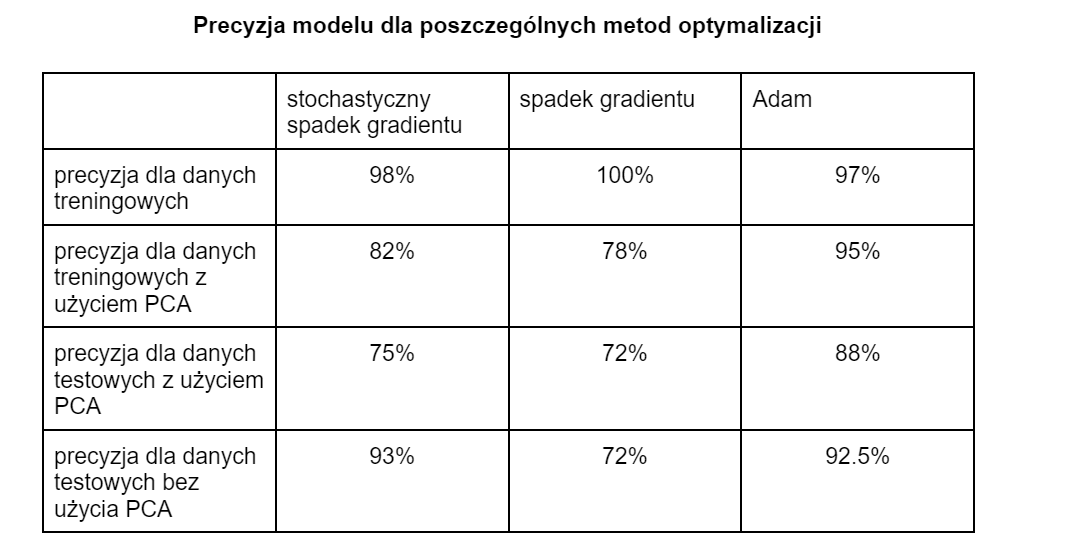
\includegraphics[width=\linewidth]{precpng.png}
jak widać w przypadku użycia metody spadku gradientu doszło do przetrenowania modelu,
mimo użytej funkcji regularyzacji.
modele zbudowane z użyciem metody Adam oraz 
metody stochastycznego spadku gradientu dały bardzo podobne do siebie wyniki,
ponieważ działają one na bardzo podobnej zasadzie. 
Użycie PCA w każdym wypadku przyczyniło się do obniżenia precyzji modelu, a tym samym do pogorszenia jego jakości.




\subsection{prdykcje modelu}
\begin{figure}[h]
  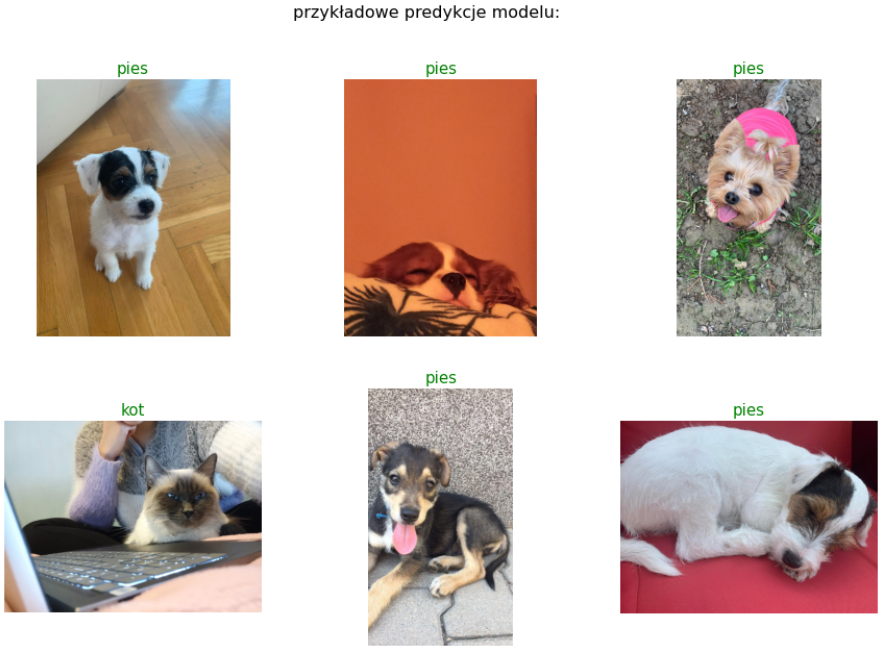
\includegraphics[width=\linewidth]{preedictions.png}
  aby zweryfikować poprawność modelu uruchomiłem go dla zdjęć zrobionych przeze mnie oraz moich znajomych,
  tak aby mieć pewność że zdjęcia są różnych formatów, rozmiarów, różnej jakości i nie 
  były wcześniej w żaden sposób przerobione
\end{figure}
model okazał się stosunkowo skuteczny, przy klasyfikacji 
zdjęć nie spreparowanych skuteczność na poziomie 93 
procent, możemy uznać za zadowalającą.\\\\
\textbf{uwaga odnośnie jakości modelu}
{dlaczego model nie ma skutecznośćci na poziomie 100 procent?}\\
\begin{enumerate}
  \item ponieważ urządzenie wykorzystane do trenowania modelu dysponuje niewielką możliwością obliczeniową,
   a operacje na zdjęciach, są skomplikowane, trenowanie sieci zakończone zostało gdy jej dokładość miała tendencje 
   rosnące.
  \item niektóre ze zdjęć mogły być nieostre, lub przedstawiać zwierzę które jest mieszanką genetyczną psa i kota.
  przykład takich zdjęć: 
  \begin{figure}[h]
    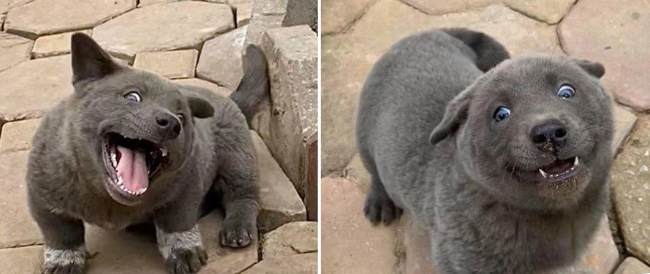
\includegraphics[width=\linewidth]{example.png}
  \end{figure}
\end{enumerate} 



\section{Wnioski}
\begin{enumerate}
  \item Wbrew informacjom, które można znaleźć w internecie użycie PCA mimo znacznego 
  zmniejszenia ilości danych procesowanych przez model 
  (w wypadku powyższego modelu 3-krotnie)
  może przyczynić się do znaczącego pogorszenia jego jakości. 
  W przypadku modelu, który procesuje uprzednio nie spreparowane zdjęcia, 
  użycie PCA nie przynosi oczekiwanych efektów.
  \item Użycie jako metody optymalizacji spadku gradientu, w każdym przypadku okazuje się mniej skuteczne od pozostałych użytych metod optymalizacji.
  nie ma więc, żadnego argumentu przemawiającego za tym by jej użyć.
  \item metoda optymalizacji Adam, choć w danym modelu okazała się nieznacznie mniej skuteczna, dla 
  dla zdjęć przetworzonych przez algorytm PCA okazała się najskuteczniejsza. Tak więc metoda ta, 
  wydaje się najstabilniejsza z metod testowanych.
  \item metoda optymalizacji stochastycznego spadku gradientu okazała 
  się najskuteczniejsza dla danych których szczegółowość była wysoka. 
  Jeśli więc model trenowany jest na szczegółowych danych jest to najlepsza metoda optymalizacji.
  \begin{figure}[h]
    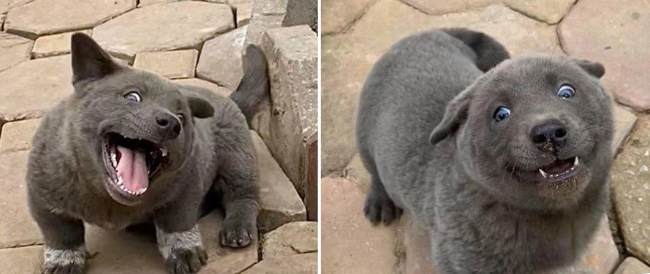
\includegraphics[width=\linewidth]{example.png}
  \end{figure}
\end{enumerate} 
\section{Przypisy}
zdjęcia użyte do budowy dla modelu:\\ 
\href{https://www.kaggle.com/datasets/zippyz/cats-and-dogs-breeds-classification-oxford-dataset}
{https://www.kaggle.com/datasets/zippyz/cats-and-dogs-breeds-classification-oxford-dataset}
kod rozwiązania:\\
\href{https://github.com/michalskibinski109/projekt/blob/main/PROJEKT.ipynb}
{https://github.com/michalskibinski109/projekt/blob/main/PROJEKT.ipynb}
\end{document}
